\chapter{Computing Trends}
\label{chapter:computing-trends}
This chapter presents the background of this thesis and motivates the need for, and the context of, efficient packet processing systems. We begin with an overview of today's challenges in hardware development, which have resulted in the transition from traditional single threaded computing to concurrent, multi-threaded and parallelized programming. Then, the dimensions of the required data processing capacity are emphasized, by explaining the concept named Big Data. Further, the characteristics of packet switched networks' data, and further the context of packet processing, i.e. cloud and fog computing, are explained.

\section{Modern Computing}
The terminology around the parallelized computation is somewhat ambiguous. Throughout this chapter, we will be using the term \emph{parallel computing} as a general term referring to the opposite of \emph{single-threaded} or \emph{sequential} computing, unless explicitly stated to mean the act of \emph{parallel computing}, in which multiple calculations are carried out \emph{simultaneously}. The general term comprises many different types of computing, such as \emph{concurrent}- and \emph{distributed computing}, as well as the type of \emph{parallel computing} itself.

\subsection{The End of Free Lunch}
\label{subsection:the-end-of-free-lunch}
Until the turn of the millennium, the main drivers for the speedups in computing were the increasing CPU clock frequency and cache sizes, as well as the execution optimizations. Faster clock speeds meant that more cycles could be run in the same time, whereas the execution optimization enabled more work to be done with the same amount of cycles. Further, the increasing cache sizes kept larger parts of the computation close to the CPU cores, away from slow shared memory.~\cite{Sutter:2005:FLiO}

A notable fact about all these drivers is that, while they lead to speedups in parallel computing, they also provide direct speedups for sequential programs. Partly for this reason, until the end of 1990s, the majority of the software applications were single-threaded and sequential.~\cite{Sutter:2005:FLiO}

However, in the mid 2000s, the CPU performance gains hit the wall. Despite the fact that the transistor densities continued following the Moore's Law~\cite{Moore:1998:MooresLaw}, several physical problems limited the development of higher clock speeds. Dennard scaling, a law proposed by in 1974 stating that the power density of transistors stays constant while the transistor themselves get smaller, seems to be broken down around 2005. As the transistors got even smaller, new current leakage and chip heating problems arose and the silicon industry hit the so-called \emph{powerwall}.~\cite{Esmaeilzadeh:2011:DSE, Sutter:2005:FLiO, Ributzka:2013:Concurrency}

\begin{figure}[]
  \begin{center}
    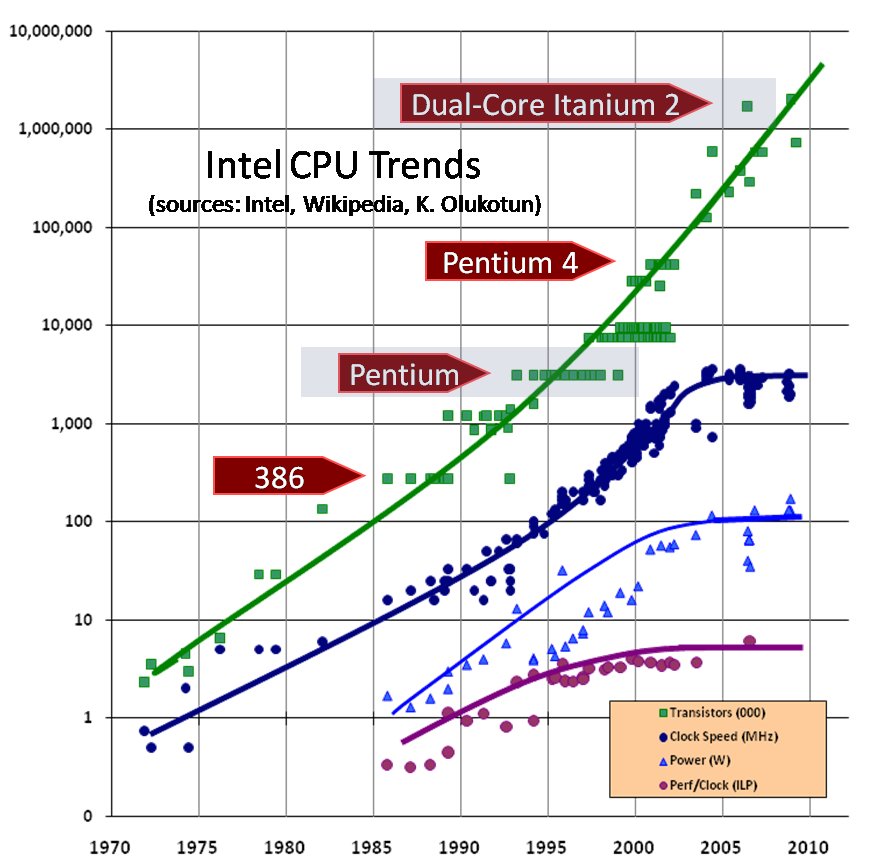
\includegraphics[width=\textwidth]{images/free-lunch-is-over.png}
    \caption{Intel CPU trends. The transistor density follows the Moore's Law, while the growth of CPU speed have stopped.~\cite{Sutter:2005:FLiO}}
    \label{fig:rne-example}
  \end{center}
\end{figure}

These chip manufacturing challenges have led into an era of \emph{dark silicon}, meaning that we cannot afford to switch all the transistors on and off at each clock cycle due to the power constraints. Before the power wall, the forefront of the silicon industry was to maximize the chip speeds. However, in the era of dark silicon, the power consumption has become perhaps the most important performance indicator, especially in the datacenter scale computing.~\cite{Sutter:2005:FLiO, Asanovic:2006:Landscape, Ributzka:2013:Concurrency, Zhang:2010:CloudComputing}

And while the silicon industry are facing various hardware development challenges, the software developers are also forced to adopt new programming paradigms to keep up with the ever increasing performance requirements.~\cite{Sutter:2005:FLiO}

\subsection{Parallel Computing}
\label{subsection:parallel-computing}

The parallelization of computing has been researched for several decades. Before the sequential execution speedup gains hit the wall, it remained a minor but important field of research, mainly in high-performance computing. Parallel-, concurrent-, and distributed computing quickly became the dominant answers for mainstream computing, to continue enjoying the benefits of the exponential computing speedups.

The \emph{parallel computing type} refers to computing in which a subparts of a program are solved at the same time. \emph{Concurrent computing}, on the other hand, executes multiple computations on overlapping time periods. In \emph{distributed computing}, the overlapping or simultaneous executions are carried out on multiple computers connected to each other.

There exist many different forms of parallel computing, often divided into four high level categories: bit-level, instruction-level, task, and data parallelism. Parallelism can be implemented in both software and hardware levels.~\cite{Culler:1997:PCA}

Bit-level parallelism refers to increasing the processor word size, thus reducing the needed number of instructions to be executed. In instruction level parallelism, the processor executes multiple instructions at the same time. Instruction level parallelism can happen in both hardware or software level.~\cite{Culler:1997:PCA}

The data parallelism refers to the simultaneous execution of the same function, on multiple cores, across the elements of the input data. Modern graphics processing units (GPU's), often implemented as wide single instruction, multiple data (SIMD) principle, are examples of data parallelism.~\cite{Culler:1997:PCA}

In contrast to data parallelism, task parallelism refers to execution of multiple cores of (possibly) completely different functions, across the same or different input data. In a typical multi-core processor, task parallelism is achieved by executing different threads or processes, on each core.~\cite{Culler:1997:PCA}

Another form of parallelism, specific to the context of network processing, is called ~\emph{Packet-level parallelism}. Network packets are typically processed on packet-by-packet basis. Most network packets are independent of each other, except for the ordering constraint for packets belonging to the same flow, thus enabling different forms of parallelism to be implemented in network processing units.~\cite{Liljeqvist:2003:Visions}

Introducing parallelism into the computing brings various new challenges in the software development. For example, the lack of a global clock, and possible failure of components demands extensive care from the developers, on top of the already challenging software development. Different frameworks and methods have been implemented, to ease the software development of efficient parallel applications. The focus of this thesis is on task level parallelism, especially in the context of packet processing applications. We will present some of the task processing frameworks more comprehensively in subsection~\ref{sec:packet-processing}.~\cite{Asanovic:2006:Landscape}

While implementing parallel systems is challenging for software developers, there are also clear limitations in the speedup gains that these methods can achieve. Amdahl's Law states the rather obvious maxima in the speedup that the program can achieve by scaling the computation over N processors. Suppose that the parallelizable proportion of a program is P (and thus the non-parallelizable proportion being P-1), then the maximum speedup, as denoted by Amdahl's Law, is:~\cite{Amdahl:1967:VSP}

\begin{equation*}
  \frac{1}{(1-P) + \frac{P}{N}}
\end{equation*}

The implication of Amdahl's Law is that the speedup of a computer program is always limited by the program's non-parallelizable proportion, thus bringing new challenges to the utilization of the available computing resources.


\section{Big Data}
\label{section:big-data}
The Internet traffic volumes are growing rapidly. For the first time, in 2010, the number of devices connected to the Internet (12.5 billion) passed the world's human population (6.8 billion). This growth is explained by the number of mobile devices (mobile phones and tablets, especially in developing countries), and the proliferation Internet of Things (IoT) devices and sensors. Cisco projects the number of mobile devices connected to the Internet, to grow up to 50 billion through 2020. IoT devices and sensors included, this number will double to over 100 billion.~\cite{Evans:2011:IoT}

According to EMC corporation sponsored IDC study~\cite{Turner:2014:Digital}, the size of the digital universe is estimated to grow ten-fold, from 4.4 zettabytes to 44 zettabytes, between 2013 and 2020. The data comes from several different sources and in many different forms. At the same time the processing requirements are growing. Everyday end users are expecting services to be delivered in higher quality near real-time, and growing number of industry, medical, and other performance critical applications are depended on the processed data.

With the enormous data masses, data diversity, and with complex processing requirements, often referred as Big Data, the traditional data processing methods become inadequate and the new performance analysis solutions become more important.


\section{Packet Processing}
\label{sec:packet-processing}

\subsection{Network Components}
Packet switching refers to a method of transmitting data in separate, suitable sized blocks, called packets, between the links of a telecommunications networks. The importance of packet switched networks is increasing in every part of the communication networks, which is explained partly by the Internet itself being an enormous packet switched network.

The Open Systems Interconnection (OSI) model is a standard conceptual model, which characterizes the communication functions involved in a general network communications of computer system. The model defines seven hierarchical layers of functional elements, between the physical interconnections (layer 1) and the software applications (layer 7).~\cite{ISO:1994:OSI}

The Internet Protocol Suite, or Transmission Control Protocol / Internet Protocol (TCP/IP), is a set of core protocols for the Internet and similar packet switched networks. It provides end-to-end data communication and specifies data packetizing, addressing, transmission, routing and receiving in the packet network. In addition to TCP and IP protocols, it provides several other network and transmission layer functionalities. The functionalities are divided into four abstraction layers: application layer, transport layer, internet layer, and link layer.~\cite{Braden:1989:TCPIP}

Internet Protocol (IP) is an essential Internet layer protocol of the Internet Protocol Suite. It provides the necessary addresses and (unreliable) delivery mechanisms for datagrams between the transmission endpoints. It is a connectionless, best-effort protocol with no error control, sequencing, or end-to-end reliability, but rather contains only the functions for packet fragmentation and delivery through the network. The packets in the IP protocol can be forwarded independent of other packets, forwarding them on-the-fly by routers.~\cite{Deering:1998:Internet}

A packet refers to the unit of data transmitted across the network. Packets consist of two parts: the header information and the payload data. Network routers use the header information to direct the packet to destination system, whereas the payload is extracted and used by the application software. All the higher layer protocols in the TCP/IP stack are encapsulated in the IP-packet's payload section.~\cite{Deering:1998:Internet}

In a conventional IP-based network architecture, the packet processing equipment and functionality is partitioned into three components: management plane, control plane, and data plane.~\cite{Chao:2007:HPS}

The control plane refers to the parts of the routing architecture, which carries and consumes the control packets needed to describe the network topology and correctly route the actual data packets. The control packets originate from and are destined for a router.~\cite{Chao:2007:HPS, Yang:2004:FCE}

The data plane, often referred as forwarding plane, deals with the actual data forwarding in the network. It defines the part of the routing architecture, which decides destination and takes action for the data arriving to it. The decision is typically determined by a look-up table, which the incoming packet is compared to. The management plane carries the traffic used for the administrative tasks of the network.~\cite{Chao:2007:HPS, Yang:2004:FCE}

\subsection{Traffic Characteristics}
The nature of the high-speed packet processing entails new types of constraints to the computing; Advanced stream processing systems are needed to process the data on-the-fly in the vicinity of the sources.~\cite{Bonomi:2012:Fog}

In the traditional von Neumann model of computing~\cite{Neumann:1993:EDVAC}, the computation is carried out by modifying the data stored in memory. However, the growing volumes of data and strict latency requirements, require not only distributing the computation, but also changes the nature of it more towards stream processing. The manipulation of the data streams passing through the system must often be done on the on-the-fly.~\cite{Bonomi:2012:Fog, Thies:2002:StreamIt}

In packet switched networks, the data streams are called \emph{flows}. Flows represent the data in specific time periods between specific network end-points. A single flow contains a large number of packets. The Internet Protocol allows each individual packet of a stream to be processed in any order, leaving the ordering of the packets to the end devices. This characteristic makes packet processing applications look like ideal for a parallel computing. However, protocols such as TCP/IP (accounting over 80\% of the Internet traffic~\cite{Fraleigh:2001:Packet}), have significant performance reductions due to reordering of packets in a single stream. For this reason, the packet processing systems often have built-in schemes, such as specialized queue management and buffering, to efficiently keep flow specific packets traversing through the queues in order.~\cite{Govind:2008:PacketReorder, Kumar:1998:RouterArchitecture}

\subsection{Networking Equipment}
Packet processing refers to the methods and concepts applied to transport data packets through the various network elements in a communication network. The network routers, switches, and other devices, such as computers and smartphones, all have their own packet processing subsystems to manage the packet traversal between the network elements. This thesis focuses on the packet routing equipment in the middle of Internet backbone.

% high performance and programmability are competing goals
% -> even mutually exclusive?

% One of the cornerstones of the Internet is the ability to connect devices together into networks, and further set of networks into internetworks. Packet switches and routers ...

% Routers and switches are the cornerstones of the Internet. They are used to connect multiple heterogeneous devices together, forming a network of devices, whereas the routers connect. heterogeneous networks into internetworks.

Traditionally, the focus in the development of network equipment -- switches, routers, and various other middleboxes -- has been to achieve high performance with very limited packet processing functionalities. The network appliances and middleboxes have typically been deployed on special purpose Application-Specific Integrated Circuits (ASIC) hardware, mainly due to high performance requirements compared to the hardware development and the absence of extensibility and flexibility requirements.~\cite{Dobrescu:2009:REP}

However, the required network functionality is becoming increasingly sophisticated. In addition to the traditional layer 2 and layer 3 routing and switching tasks, the network elements are required to handle more demanding tasks (e.g. application acceleration, encryption, and intrusion detection) all the way to layer 7. These extensions often require modified per-packet processing on the router data plane, and as the specialized network processors are difficult to extend and program, both industry and research are seeking new, more flexible networking solutions.~\cite{Egi:2009:PP, Dobrescu:2009:REP}

On the other extreme of the design spectrum, are the software routers built from general-purpose operating systems and x86 hardware platforms. The main promise of the software routers is their extensibility in the software and hardware development: the system's network functionalities, both in the data and control plane, can be modified fully by the software, thus mitigating the hardware design and development burden of the network developers.~\cite{Dobrescu:2009:REP}

The software routers also enable several other properties of the general purpose computer ecosystem. Huge manufacturing volumes and widespread supply and support chain allow much cheaper hardware prices. The rapid advances in commodity semiconductor technology, such as the state-of-the-art power management features, can provide significant advantages over the slow hardware upgrade cycles of the traditional ASIC based systems.~\cite{Dobrescu:2009:REP}

The challenge with the full software routers is the scaling the approach to high-speed networks. Between these two extremes exist design solutions, which offer much of the programmability of commodity hardware and the performance of specialized ASIC systems. Our focus in this thesis, is on the MPSoC systems consisting of these middle ground network processing units.~\cite{Dobrescu:2009:REP}

\section{Virtualization}
\label{section:virtualization}
Virtualization is an act of dividing a common set of computing resources into a multiple isolated execution environments. It enables multiple operating systems to be run, in parallel, on a single processing unit, thus alleviating the efficiency problems of parallel computing.

Before the existence of multi-user operating systems and the rapid drop in hardware cost around 1980s, the virtualization was used to allow multiple users to share the same mainframe hardware. Until the end of 1990s, it remained mainly a practice of computing industry and academic research, often requiring special hardware with explicit support for virtualization. VMWare's introduction of virtualization to the x86 architecture~\cite{Walters:1999:VVP} and the personal computer industry introduced the benefits of virtualization to the wider masses.~\cite{Bugnion:2012:BVX, Barham:2003:XAV}

\subsection{Platform Virtualization}
In the traditional, non-virtualized system, the hardware platform resources are controlled by a single operating system. Virtualization introduces a new layer, the \emph{hypervisor} (also referred as virtual machine monitor), to the software stack. The hypervisor lies underneath the existing software components, abstracting the hardware inputs, outputs, and the behavior for the use of multiple operating systems. The virtualized system is called a \emph{virtual machine}.~\cite{Uhlig:2005:IVT, Bugnion:2012:BVX, Barham:2003:XAV}

The benefits of the virtualization are numerous, mainly due to the software implementation of the virtual machines. It enables scalability and flexible migration of computation loads across different infrastructures, leading to improved hardware utilization, dynamic resource allocation and management, isolation, security, and automation.~\cite{Pearce:2013:VIS}

The virtual machines can be \emph{live migrated} over to another physical machine. While the non-virtualized systems are often under utilized, the flexibility of software enables the machines often to be run on optimal usage level. Maintenance costs can be reduced by software automation and security can be increased by additional software services, such as workload isolation. These benefits have encouraged companies to seek savings, by adopting virtualization in various contexts, ranging from the desktops and datacenters to network switching.~\cite{Uhlig:2005:IVT, Pearce:2013:VIS}

To enable fully functional virtualized environments, the virtualization of different system components, such as CPU, memory, I/O, and storage, need to be considered. CPU virtualization techniques are often divided into three categories: binary translation (full virtualization), paravirtualization, and hardware-assisted virtualization.~\cite{Bugnion:2012:BVX, Pearce:2013:VIS, Horne:2007:Understanding}

Full virtualization refers to a method where the communication between the virtualized operating system (guest) and the underlying host operating system is (nearly) completely emulated, meaning that the virtual hardware is functionally identical to the underlying machine. Unmodified guest operating systems can be run similarly as on native hardware, as the virtualization layer completely decouples them from the underlying hardware. On the other hand, the complete emulation of the hardware instructions induces performance overhead to the full virtualization.~\cite{Bugnion:2012:BVX, Barham:2003:XAV, Horne:2007:Understanding}

In paravirtualization, instead of emulating the hardware environment, the guest operating systems are executed in isolated environments. It enables the communication between the guest operating system and the hypervisor, and thus improving the performance and efficiency of the virtualization.~\cite{Barham:2003:XAV, Horne:2007:Understanding}

However, paravirtualization requires modifying the guest operating system kernel to enable direct communication with the virtualization layer monitor. For this reason, paravirtualization compatibility and portability is limited, and it can cause significant support and maintainability costs.~\cite{Barham:2003:XAV, Horne:2007:Understanding}

Hardware assisted virtualization introduces new hardware features to ease the virtualization. A common method is to provide a new privilege level below the ring 0, to allow the guest operating system to intercept and emulate privileged operations of the underlying hardware. Hardware assisted virtualization removes the need for binary translation and paravirtualization, thus, at least theoretically, solving many of the current virtualization problems.~\cite{Horne:2007:Understanding, Pearce:2013:VIS}

\subsection{Operating System Level Virtualization}
Running multiple operating systems on single hardware, as done with hypervisor-based virtualization, comes with the cost of efficiency. In many scenarios, such as high performance computing, game hosting, or MapReduce~\cite{Dean:2008:MR}, the overhead from running multiple kernels on the same machine becomes a problem. Another common method for server virtualization is to run the virtualization layer within the operating system.~\cite{Soltesz:2007:COS, Xavier:2014:Containers}

Operating system level virtualization is based on the kernel's ability to support multiple isolated user-space instances, or software \emph{containers}. Instead of emulation, programs running in containers consume the host operating system's standard system call interface, resulting in negligible virtualization overhead compared to hypervisor-based virtualization. The drawback of container based virtualization is its inflexibility; each guest must be running on the same operating system kernel as the host machine.~\cite{Soltesz:2007:COS, Xavier:2014:Containers}

Examples of operating system level virtualization implementations include for example Linux Containers (LXC)~\cite{LinuxContainers:2013:LXC}, Linux-VServer~\cite{Des:2005:Virtualization}, OpenVZ~\cite{OpenVZ:2013}, and Docker~\cite{Merkel:2014:Docker}. While most of the container implementations seem to achieve near-native performance, the management capabilities, such as, performance isolation, vary between them.

\section{Cloud Computing}
Cloud computing paradigm provides a shared pool of easily configurable and flexible computing resources via convenient, on-demand network access. One of the driving forces for cloud computing has been its promise of economics of scale. Virtualization techniques enable cloud computing centers, compared to traditional on-premise solutions, to be built using cheaper hardware, cooling, electricity, network capacity and smaller number of administrators per computer. At the same time, it alleviates the problem of inefficient resource usage, caused by the challenges discussed in section~\ref{subsection:the-end-of-free-lunch}.~\cite{Mell:2011:ccdef}

According to the definition of The National Institute of Standards and Technology, cloud computing is composed of five essential characteristics (on-demand self-service, broad network access, resource pooling, rapid elasticity, and measured service), three service models (software as a service, platform as a service, and infrastructure as a service), and four deployment models (private cloud, public cloud, community cloud, and hybrid cloud).~\cite{Mell:2011:ccdef}

%\subsection{Characteristics}
The \emph{on-demand self-service} characteristic means that the consumer of the service can provision computing resources, such as server time and network storage, automatically without requiring human interaction with each service provider. \emph{Broad network access} requires the service to be available over the network and accessible using standard mechanisms which promote use by heterogeneous platforms such as mobile phones, tablets, laptops, or personal computers. \emph{Resource pooling} refers to virtualization techniques discussed in the subsection~\ref{subsection:virtualization}. \emph{Rapid elasticity} means that the consumer is able to elastically and automatically, provision and release the seemingly unlimited resources on demand. The last characteristic, \emph{measured service}, refers to the automatic control and optimization of the resources by metering the usage of the services.~\cite{Mell:2011:ccdef}

The characteristics of cloud computing make it tempting for both customers and service providers. From the customer perspective, it provides advantages of high computing power, cheap service costs, high performance, flexible scalability and accessibility as well as high availability. It reduces the upfront infrastructure costs for companies, allowing them to focus on their core businesses instead of on infrastructure, and getting their applications running faster, with improved manageability and less maintenance. On the other hand, it provides completely new business models for the service providers.~\cite{Mell:2011:ccdef, Dikaiakos:2009:Cloud}

%\subsection{Service Models}
The three service models divide the cloud services into logical levels based on the computing layers provided by the cloud service. Figure~\ref{fig:cloud-computing-service-models} presents the comparison these levels together with the on-premise solution. On-premise solution refers to model where the customer manages the complete computation stack.

\begin{figure}[]
  \begin{center}
    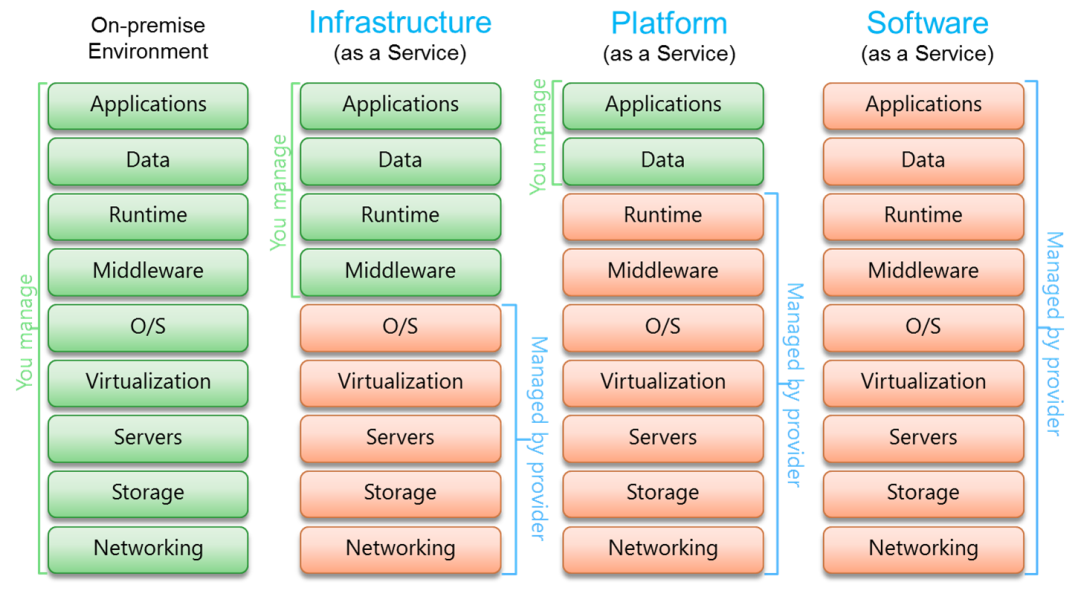
\includegraphics[width=\textwidth]{images/cloud-computing-service-models.png}
    \caption{A comparison of the three cloud service models and on-premise solution. Figure from~\cite{Lau:2011:ServiceModels}}
    \label{fig:cloud-computing-service-models}
  \end{center}
\end{figure}

The lowest of the three levels, \emph{Infrastructure as a service (IaaS)} model, provides the customer the services which abstract the details of typical hardware resources and operating systems. The computing resources are typically abstracted using a hypervisor, such as VirtualBox, KVM, Hyper-V that runs the virtual machines visible to customers as guests. Examples of IaaS providers are Amazon Web Services~\cite{Murty:2008:AWS} and Rackspace~\cite{Rackspace:2010:Inc}.~\cite{Mell:2011:ccdef}

In the next service level, \emph{Platform as a service (PaaS)} model, the service provider takes care of the platform-level middleware and runtime components. These components typically include programming-language execution environment, databases, and web servers. Google AppEngine~\cite{Sanderson:2009:GoogleAppEngine} and Windows Azure Platform~\cite{Redkar:2011:Azure} are examples of PaaS providers.~\cite{Mell:2011:ccdef}

\emph{Software as a service (SaaS)} model provides, on top of the IaaS and PaaS, the management of the application and data level. The customers access the software from cloud clients, typically web browsers via personal computers, laptops, tablets or smartphones. SaaS has become a common model for delivering wide range of different applications, such as Facebook~\cite{facebook}, Salesforce~\cite{salesforce}, and Google Gmail~\cite{Teeter:2011:Gmail}.~\cite{Mell:2011:ccdef}

%\subsection{Deployment Models}
\emph{Private Cloud} infrastructure is hosted internally by a company or organization, targeting a specific set of customers. Private clouds are typically more affordable to setup and offer more flexibility, while also providing the companies full privacy on their data and applications. \emph{Public Cloud}, on the other hand, is exposed to any customer over a public network. The data, applications and other resources are stored over the service provider's data center, and thus the security has to be considered. The underlying infrastructure is often similar between these two models.~\cite{Mell:2011:ccdef}

The cloud service can also be a combination of the public and private clouds. This kind of deployment model is referred to as a \emph{hybrid cloud}. Hybrid cloud allows the utilization of the flexibility and cost of the public cloud solutions, while at the same time maintaining the security sensitive data in their own infrastructure. \emph{Community cloud} refers to cloud infrastructure that is shared between multiple organizations, typically with common security, jurisdiction, and compliance concerns in mind. Community clouds can be hosted and managed either internally or externally from the sharing organizations.~\cite{Mell:2011:ccdef}

\subsection{Energy Consumption}
The power consumption has become the major concerns in the design of today's warehouse scale datacenters. In 2005, the world's server power demand (including cooling and auxiliary infrastructure) was about 14,000MW, resulting in about \$7.2B eletcricity costs. Majority of these costs come from cooling, which is the consequence of the heat generated by the computing resources such as CPU, memory, storage, and networking.~\cite{Koomey:2007:PC, Fan:2007:PPW}

Virtualized datacenters can greatly increase the usage rates of computing resources, decreasing the total server energy consumption. However, the benefits of cloud computing are tightly coupled to the scale of the individual datacenters. While the total energy consumption is reduced, the energy usage of individual datacenters are often huge.~\cite{Hoelzle:2009:DCI}

The datacenter costs can be optimized by more efficient hardware implementations and increased usage rates, but companies also have to consider different non-technical solutions. The design and construction of warehouse scale datacenters should be treated similarly to traditional factories. Size, location, and physical design of the datacenter can have considerable effect on the costs.~\cite{Hoelzle:2009:DCI}

Google's Summa datacenter is a good example of the scale of the cloud datacenter. Google, a company residing in California, invested over \$200M to build a datacenter in Hamina, Finland. The benefits from Finland's energy infrastructure, cold climate, developable land and available workforce, outweighed all the negative qualities of building the datacenter on the other continent, nearly 9000km away from the company's head quarters.~\cite{Google:2016:Summa}

\subsection{Datacenter Networks}
For compatibility and cost reasons, datacenter networks are often built from commodity Ethernet switches and routers (scaling out), rather than from expensive high-end hardware (scaling in). Due to the limits in the switch port densities even in the high-end hardware, the traditional single rooted topologies are replaced with multi-rooted tree topologies such as fat-tree or leaf-spine. Multi-rooted network design allows to scale the data center networks' bisection bandwidth by adding new spine switches into the network.~\cite{Al-Fares:2010:SO, Al-Fares:2008:SCD}

Cloud computing datacenters can consist of hundreds of thousands of servers, supporting large variety of services, such as high performance computing, MapReduce~\cite{Dean:2008:MR} and web services. Many of these applications have several inter-dependent components divided across the servers. Thus, the inter-node network bandwidth has become the major bottleneck in data centers.~\cite{Al-Fares:2008:SCD}

To efficiently utilize datacenter resources, and to answer the required performance guarantees, efficient network traffic load balancing mechanisms are needed. Several different proposals, such as CONGA~\cite{Alizadeh:2014:Conga},  Presto~\cite{He:2015:Presto}, and Hedera~\cite{Al-Fares:2010:Hedera}, have been made to overcome the issues of traditional hash based schemes.

\section{Fog Computing}
\label{section:fog-computing}

% The IT and Telecommunication Networking evolutions are coming closer to each other.
% -> new possibilities
% -> computation is moving to the network edge, closer to the end user and sensors.

% ``Mobile-edge Computing can be seen as a cloud server running at the edge of a mobile network and performing specific tasks that could not be achieved with traditional network infrastructure. Machine-to-Machine gateway and control functions are one example, but there are many others.''

% ``Move the computation code to the data, not the other way''

While the benefits of Cloud Computing provide efficient alternative to the traditional on-premise solutions, there are certain issues, which have to be addressed to enable a new breed of ever demanding applications and services. Characteristics, such as mobility, geo-distribution, location awareness and low latency are intractable to achieve due to the centralized nature of cloud computing. The proliferation of devices and sensors have led to a situation where the data are produced faster than can be transmitted or stored.~\cite{Bonomi:2012:Fog, Vaquero:2014:FYW}

Fog computing is an extension to the traditional cloud computing architecture, where parts of the cloud computing services, mainly computation, storage, and networking, are carried out in the edge of the communication network. It is defined to provide the following characteristics on top of the existing cloud computing architectures: low latency and location awareness; wide-spread geographical distribution; mobility; very large number of nodes, predominant role of wireless access, strong presence of streaming and real time applications, heterogeneity.~\cite{Bonomi:2012:Fog}

High virtualization and efficient stream processing are the key elements for successful fog computing.

Until recently, the typical network architectures have been implemented on proprietary or special purpose hardware. The growing networking traffic and competition in communication services have led to the development of software based solutions. Software based solutions enable flexible and extensible networking, and measure up the tight standards for stability, protocol adherence, and quality, previously achieved only with the hardware solutions.~\cite{Kim:2013:SDN}

The main enabling technologies of fog computing are the software-defined networking (SDN), and further the network functions virtualization (NFV). Software defined networking separates the data plane and the control plane functionalities of the network, making the data plane switches simple packet forwarding devices, while leaving the routing decision control logic for the control plane. Thus the network control becomes directly programmable, centrally managed, programmatically configurable, and vendor agnostic, amongst many other benefits from softwareization.~\cite{Kim:2013:SDN}

SDN is often complemented with network functions virtualization. In NFV, the network devices are virtualized (using similar techniques as discussed in section~\ref{section:virtualization}) and the network functionalities of the devices are implemented in software packages.~\cite{Demestichas:2013:NFV}

Long Term Evolution (LTE)~\cite{Sesia:2009:LTE} and Evolved Packet Core (EPC) work as a natural platforms for the fog's edge data centers. Small cloud stations can be deployed to the EPCs, and the routers can be utilized as the virtualization infrastructure. This also enables the application services to be co-located where needed.~\cite{Vaquero:2014:FYW}

%%% Local Variables:
%%% mode: latex
%%% TeX-master: "thesis-hartikainen"
%%% End:
